\documentclass[11pt,a4paper]{article}

\usepackage[spanish]{babel}
\usepackage{amsmath,amsfonts, amssymb, mathtools} % Podemos añadir amssymb, amsthm o bm
\usepackage{graphicx, xparse}
\usepackage[top=2cm,bottom=2cm,left=3cm,right=3cm,marginparwidth=1.75cm]{geometry} % Este paquete permite modificar los márgenes del documento
\usepackage[colorlinks=true, allcolors=blue]{hyperref} % Se indica que los hipervínculos van todos en azul
\usepackage{setspace}
\usepackage{xcolor, tcolorbox, booktabs, multirow, colortbl}
\usepackage{cancel} %tachar cosas
\tcbuselibrary{breakable}
\usepackage{hyperref}
\usepackage{titlesec}
\usepackage{array}
\usepackage{tikz}
\usetikzlibrary{positioning,shapes.geometric,fit,backgrounds}
\usepackage{listings, lstautogobble}
\usepackage[T1]{fontenc}
\usepackage[utf8]{inputenc}
\usepackage{fontspec}
\usepackage{makecell}
\usepackage{nicematrix}

\newfontfamily\myfont{Consolas}

\graphicspath{ {images/}}


% \lstset{
%     language=myAssembly,
%     inputencoding=utf8,
%     basicstyle=\ttfamily\footnotesize,
%     stringstyle=\ttfamily\color{verdeSuave},
%     commentstyle=\ttfamily\itshape\color{gray},
%     emph={IS, NULLS, ROW, OFFSET, FETCH, WITH, TIES, PERCENT, REFERENCES, TRUNCATE, ADD_MONTHS, LAST_DAY, MONTHS_BETWEEN, NEXT_DAY, ROUND, TRUNC, EXTRACT, TO_CHAR, TO_DATE, TO_NUMBER, MERGE},
%     emphstyle={\color{blue}\bfseries},
%     keywordstyle=\color{blue}\bfseries,
%     morekeywords={SELECT, FROM, WHERE, INSERT, INTO, VALUES, UPDATE, SET, DELETE, JOIN, ON, CREATE, TABLE, DROP, ALTER, ADD, PRIMARY, KEY, FOREIGN, REFERENCES, CONSTRAINT, AND, OR, NOT, NULL, AS, DISTINCT, GROUP, BY, ORDER, HAVING, IN, BETWEEN, LIKE, IS},
%     numbers=left,
%     numberstyle=\tiny\color{gray},
%     xleftmargin=10pt,
%     frame=shadowbox,
%     breaklines=true,
%     extendedchars=true,    % Habilitar caracteres extendidos
%     autogobble=true,
%     tabsize=4, % Cambia el tamaño del tabulador aquí
%     literate=%
%         {á}{{\'a}}1 {é}{{\'e}}1 {í}{{\'i}}1 {ó}{{\'o}}1 {ú}{{\'u}}1
%         {Á}{{\'A}}1 {É}{{\'E}}1 {Í}{{\'I}}1 {Ó}{{\'O}}1 {Ú}{{\'U}}1
%         {ñ}{{\~n}}1 {Ñ}{{\~N}}1
% }



%Colores
\definecolor{blanco}{HTML}{FFFFFF}
\definecolor{negro}{HTML}{000000}
\definecolor{azulSuave}{HTML}{6ac9d5}
\definecolor{naranjaSuave}{HTML}{d5956a}
\definecolor{verdeSuave}{HTML}{6ad578}
\definecolor{verdeHoja}{HTML}{006400}
\definecolor{naranjaDuro}{HTML}{bd2d0e}



\titleformat{\part}[display]
  {\normalfont\Huge\bfseries} % Estilo del texto
  {}           % Prefijo antes del título de la parte
  {20pt}                      % Separación entre "Parte I" y el título
  {\Huge}                     % Estilo del título de la parte



%Colores
\definecolor{blanco}{HTML}{FFFFFF}
\definecolor{negro}{HTML}{000000}
\definecolor{azulSuave}{HTML}{6ac9d5}
\definecolor{naranjaSuave}{HTML}{d5956a}
\definecolor{verdeSuave}{HTML}{6ad578}
\definecolor{magenta}{HTML}{FF00FF}
\definecolor{dorado}{HTML}{ad8a1f}
\definecolor{amarilloPastel}{RGB}{255, 249, 196} % Amarillo pastel claro
\definecolor{amarilloOscuro}{RGB}{253, 216, 100}  % Amarillo más oscuro
\definecolor{grisSuave}{RGB}{230, 230, 230}      % Gris suave
\definecolor{negro}{RGB}{0, 0, 0}                % Negro puro

\newtcolorbox{dem_box}[1]{
before=\par\smallskip\centering,
colframe=azulSuave!70,
colback=white,
fonttitle=\bfseries,
coltitle=negro,
title=#1,
flushleft title,
width=1\linewidth,
breakable = true
}

\newtcolorbox{ejem_box}[1]{
before=\par\smallskip\centering,
colframe=verdeSuave!70,
colback=white,
fonttitle=\bfseries,
coltitle=negro,
title=#1,
flushleft title,
width=1\linewidth,
breakable = true
}

\newtcolorbox{ej_box}[1]{
before=\par\smallskip\centering,
colframe=naranjaSuave!70,
colback=white,
fonttitle=\bfseries,
coltitle=negro,
title=#1,
flushleft title,
width=1\linewidth,
breakable = true
}

\newtcolorbox{mod_box}[1]{
before=\par\smallskip\centering,
colframe=amarilloOscuro!85,
colback=amarilloPastel!30,
fonttitle=\bfseries,
coltitle=negro,
title=#1,
flushleft title,
width=0.94\textwidth,
breakable = true
}



\setstretch{1.2}
\decimalpoint

% \title{\textbf{BASES DE DATOS: } EJERCICIOS RESUELTOS}
% \author{Diego Díaz Mendaña}
%\date{Fecha}

\begin{document}

\begin{titlepage}
    \begin{center}
        % Logo de la institución
        
\includegraphics[width=0.3\textwidth]{logo_escuela.png} \\[1cm] % Cambiar logo_escuela por el nombre del archivo con el logo
        \vspace{1cm}
        
        \textbf{\LARGE ESCUELA DE INGENIERÍA INFORMÁTICA DE OVIEDO} \\[1.5cm]
        
        \rule{\linewidth}{0.5mm} \\[0.4cm]
        \textbf{\Huge Fundamentos de Computadores Y Redes} \\[0.3cm]
        \rule{\linewidth}{0.5mm} \\[1cm]
        
        {\Large Curso 2024-2025} \\[1.5cm]
        
        \textbf{\LARGE Trabajo Grupal - Fase I} \\[0.8cm]
        
        \text{Díaz Mendaña, Diego - UO301887}\\[0.15cm]
        \text{García Pernas, Pablo - UO300167}\\[0.15cm]
        \text{Gota Ortín, Jorge - UO301023}\\[0.15cm]
        \text{Suárez Fernández, Fernando - UO300028}
        
        \vfill
        
        % Información del alumno
        \begin{flushright}
            \textbf{Grupo de prácticas:} PL.3 - A \\[0.3cm]
            \textbf{Titulación:} PCEO Informática y Matemáticas \\[0.3cm]
        \end{flushright}
        
        \vfill
        
        \today \\[1cm]
    \end{center}
  \end{titlepage}

\newpage
\hypersetup{linkcolor=black}
\tableofcontents
\hypersetup{linkcolor=blue}
\newpage

\section{Introducción}
La presente memoria da cuenta del desarrollo de la Fase I del trabajo práctico correspondiente a la asignatura Fundamentos de Computadores y Redes, con el propósito de profundizar en los conceptos generales tratados en los laboratorios de la citada asignatura. A través de la implementación de un sistema de control de licencias parametrizado, se integran conocimientos relativos al lenguaje \texttt{C/C++} y al ensamblador sobre arquitectura \texttt{Intel x86-64}, abordando aspectos fundamentales como el manejo de bits, máscaras, desplazamientos y estructuras de control.\vspace{3ex}



\section{ID}
Para el desarrollo del presente proyecto se ha seleccionado como identificador de referencia el número \textit{UO300028}, al ser el más bajo entre los disponibles dentro del grupo, conforme a lo estipulado en la guía oficial de la práctica. No obstante, cabe señalar que, en determinados fragmentos del código —como se detallará en secciones posteriores de esta memoria—, se ha optado por la utilización de identificadores alternativos. Esta decisión ha respondido a la necesidad de preservar la coherencia lógica y funcional del programa, la cual se veía comprometida al emplear un único identificador de forma estricta en todos los contextos del desarrollo.
\vspace{3ex}

\section{Desarrollo del programa}
\subsection{Descripción general}
El programa desarrollado consiste en un sistema simplificado de control de licencias, parametrizado mediante un identificador numérico asociado al número de matrícula universitaria. Su implementación combina el lenguaje \texttt{C++}, utilizado para la lógica principal y la gestión de entrada/salida, con código en ensamblador \texttt{x86-64} para una función específica de validación. Todo el desarrollo se ha realizado en el entorno \textit{Visual Studio}, respetando la configuración proporcionada por la asignatura (\texttt{Teamwork}).



\subsection{Funciones implementadas}
\subsubsection{\texttt{ControlWithReversedStrings()}}
La función implementada tiene por objeto la verificación del formato de dos cadenas introducidas por el usuario a través de la consola, conforme a los criterios establecidos en el enunciado de la práctica. Para la inversión de la segunda cadena, se ha recurrido a la función nativa \texttt{strrev()}, propia del lenguaje \texttt{C++}, lo que permite una manipulación directa y eficiente de las estructuras de texto. A continuación, se muestran sendos ejemplos de entrada válida e inválida:
\begin{itemize}
  \item \textbf{Entrada válida:} \texttt{aaaaaaaaaaaaaa} y \texttt{1df4g7n9}
  \item \textbf{Entrada inválida:} \texttt{a} y \texttt{a}
\end{itemize}

\vspace{3ex}

\subsubsection{\texttt{MaskControl()}}
\textcolor{naranjaDuro}{Dado que el identificador asignado inicialmente (300028) conducía a una interpretación no operativa de la condición planteada —al implicar, en la práctica, la selección de los 32 bits menos significativos del segundo y los 0 bits más altos del primeros, resultando en el uso exclusivo del segundo operando—, se ha optado por emplear de forma justificada el identificador alternativo 299928, con el fin de preservar la lógica y coherencia funcional del ejercicio.} \vspace{2ex}

\noindent La función en cuestión verifica el formato de dos valores enteros introducidos por consola, conforme a los criterios específicos establecidos en el guión de la práctica. A continuación, se muestran sendos ejemplos de entrada válida e inválida:
\begin{itemize}
  \item \textbf{Entrada válida:} \texttt{1024} y \texttt{32315}
  \item \textbf{Entrada inválida:} \texttt{0} y \texttt{0}
\end{itemize}
\vspace{2ex}

\noindent Alternativamente, se ha valorado la opción de realizar este ejercicio empleando máscaras de bits, en lugar de emplear desplazamientos de bits. El código correspondiente a esta implementación se muestra a continuación: \vspace{2ex}
\begin{center}
  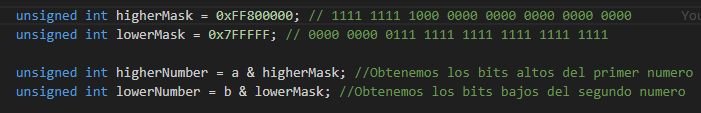
\includegraphics[width=1\textwidth]{alternativaPablo.png}
\end{center}

\vspace{3ex}

\subsubsection{\texttt{ControlInAsm()}}
\textcolor{naranjaDuro}{Dado que el identificador asignado inicialmente (300028) conducía a una interpretación no operativa de la condición planteada —al implicar, en la práctica, que los 0 bits más bajos tenían que ser mayores a 108, lo cual es imposible—, se ha optado por emplear de forma justificada el identificador alternativo 299928, con el fin de preservar la lógica y coherencia funcional del ejercicio.} \vspace{2ex}

\noindent La función realiza una verificación inicial en \texttt{ensamblador} sobre los 9 bits menos significativos de un valor de 32 bits introducido por consola. En caso de superar dicha validación, se procede a efectuar una segunda comprobación lógica entre los otros dos valores también recibidos por consola. A continuación, se muestran sendos ejemplos de entrada válida e inválida:
\begin{itemize}
  \item \textbf{Entrada válida:} \texttt{111}, \texttt{0} y \texttt{0}
  \item \textbf{Entrada inválida:} \texttt{0}, \texttt{0} y \texttt{0}
\end{itemize}
\vspace{3ex}

\subsubsection{\texttt{CheckArray()}}
La función toma tres valores de entrada, que se almacenan en un array de tres elementos de 8 bits. Se realiza una operación \texttt{AND} a nivel de bit entre los tres valores, y si el resultado —interpretado en base decimal— difiere de 200, se muestra un mensaje de error y se interrumpe la ejecución. A continuación, se muestran sendos ejemplos de entrada válida e inválida:
\begin{itemize}
  \item \textbf{Entrada válida:}  {\myfont ╚ ╚ ╚}
  \item \textbf{Entrada inválida:} \texttt{z z z}
\end{itemize}

\vspace{3ex}

\section{Cuestiones}
A continuación se presentan las respuestas a las cuestiones planteadas en el guión de la práctica. \vspace{2ex}

\subsection{Cuestión 1}
En la siguiente imagen se muestra el código en ensamblador correspondiente al paso de parámetros y llamada de la función \texttt{isValidAssembly()} desde \texttt{ControlInAsm()}. Para llegar a él, se ha empleado la opción de depuración de \textit{Visual Studio} llamada \texttt{desensamblado} activando la opción \textit{mostrar bytes de código}:\vspace{2ex}
\begin{center}
  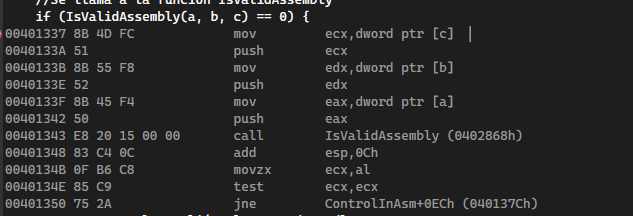
\includegraphics[width=1\textwidth]{pasoParametrosCodigo.png}
\end{center}
\vspace{3ex}

\noindent A partir de la imagen, podemos ver que el paso de parámetros se realiza en la dirección de memoria \texttt{00401337} y la llamada al procedimiento en \texttt{00401343}. Dado que el enunciado destila cierta ambigüedad en cuanto al código requerido, se ha optado por añadir también el código de la función \texttt{isValidAssembly()}: \vspace{2ex}

\begin{center}
  \begin{minipage}{0.49\textwidth}
      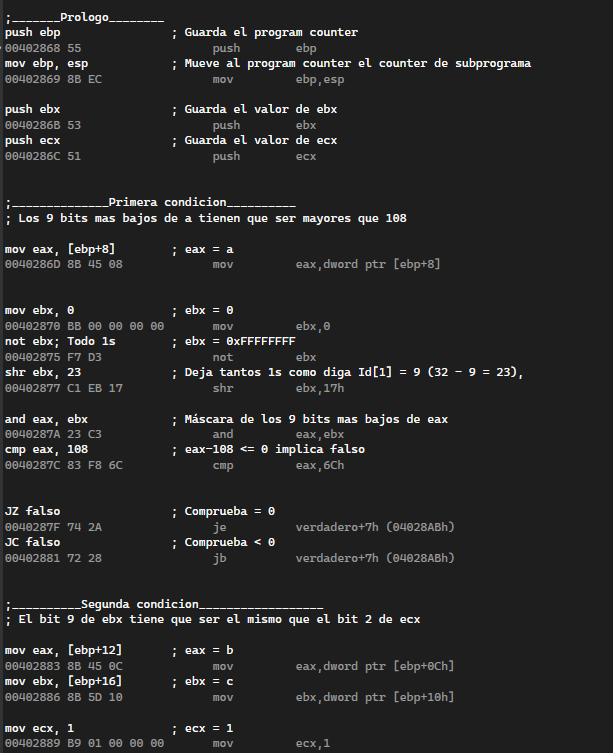
\includegraphics[width=1.055\textwidth]{isValidAssembly1.png}
  \end{minipage}
  \begin{minipage}{0.49\textwidth}
      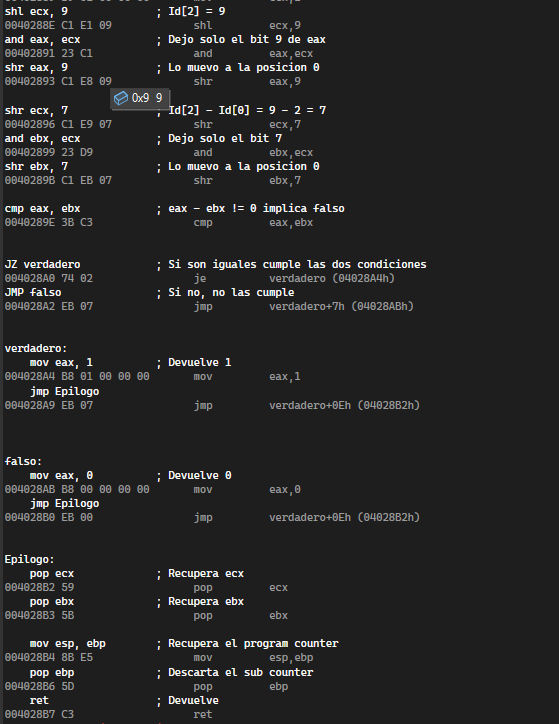
\includegraphics[width=1\textwidth]{isValidAssembly2.png}
  \end{minipage}
\end{center}
\vspace{2ex}

\subsection{Cuestión 2}
Empleando las herramientas de depuración de \textit{Visual Studio} (depurador, ventana de memoria, etc.), se ha procedido con la ejecución del programa y, tras pasar la primera cadena de caracteres y llegar al \texttt{breakpoint} correspondiente, se ha analizado la dirección de memoria en la que se almacena el array de caracteres. Dicha posición de memoria es \texttt{0x0019FECC}, como se muestra en la siguiente captura de pantalla: \vspace{2ex}
\begin{center}
  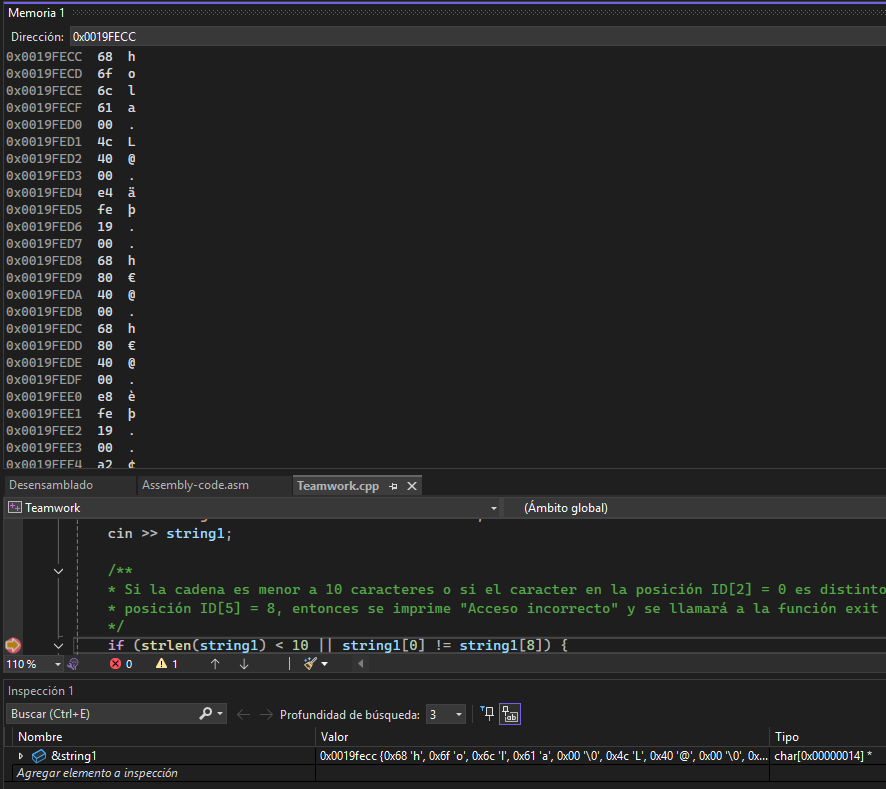
\includegraphics[width=0.82\textwidth]{direccionMemoriaCWRS.png}
\end{center}
\vspace{3ex}

\subsection{Cuestión 3}
Se han empleado las herramientas de depuración de \textit{Visual Studio} (depurador, ventana de memoria, ventana de registros, ventana de desensamblado, etc.) para analizar el contenido de los registros y la pila en el momento de la llamada a la función \texttt{CheckArray()}. Se ha comprobado el valor \texttt{EBP} en la ventana de registros y en la de memoria y la dirección de retorno con la ventana de desensamblado y la de memoria. A continuación, se muestra una captura de pantalla con los resultados obtenidos:
\begin{center}
  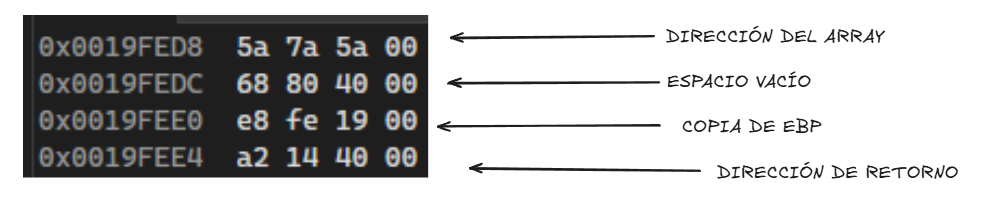
\includegraphics[width=1\textwidth]{retornoFuncion2.png}
\end{center}

\noindent Notar que las direcciones de retorno se dan en formato \textit{little-endian}, por lo que la dirección de retorno es \texttt{0x004014A2}. \vspace{3ex}
\vspace{3ex}

\subsection{Cuestión 4}
Para la realización de esta cuestión, se ha empleado la herramienta de desensamblado de \textit{Visual Studio} para analizar el código ensamblador de la función \texttt{CheckArray()}. A continuación, se muestra una captura de pantalla con el código ensamblador de la función en cuestión: \vspace{2ex}
\begin{center}
  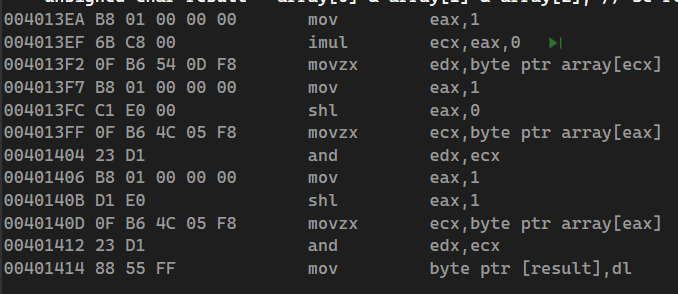
\includegraphics[width=1\textwidth]{codigoEnsambladorCheckArray.png}
\end{center}
\vspace{2ex}

\noindent A partir de la imagen, se puede ver el código correspondiente a la línea en la que se realiza la operación \texttt{AND} a nivel de bit entre los tres valores introducidos por el usuario:
\begin{itemize}
  \item \texttt{MOV eax, 1}: Mueve el valor 1 al registro \texttt{EAX}.
  \item \texttt{IMUL ecx, eax, 0}: Multiplica el valor de \texttt{EAX} por 0 y lo almacena en \texttt{ECX}.
  \item \texttt{MOVZX edx, byte prt array[ecx]}: Mueve el valor de \texttt{array[0]} al registro \texttt{EDX}. Ya que se trata de un byte, se rellena con ceros a la izquierda.
\end{itemize}

\vspace{3ex}

\vspace{3ex}
\section{Distribución del trabajo}
\subsection{Estrategia de trabajo}
La implementación del proyecto se ha organizado siguiendo una estrategia de trabajo colaborativo, basada en la asignación individual de cada una de las funciones principales descritas en el enunciado. Cada integrante del grupo asumió la responsabilidad del desarrollo, depuración y validación de una función específica, lo que favoreció una distribución equilibrada de las tareas y una mayor especialización técnica en cada componente del sistema. \vspace{2ex}

\noindent Como soporte para el trabajo en equipo, se ha utilizado el sistema de control de versiones distribuido \textit{Git} en combinación con la plataforma \textit{Github} como repositorio remoto centralizado. El grupo ha adoptado un flujo de trabajo basado en la estrategia de \textit{feature branching}, en la cual cada funcionalidad fue desarrollada en una rama independiente derivada de la rama principal \texttt{main}. Una vez finalizada la implementación de cada funcionalidad, se procedía a la apertura de una \texttt{pull request (PR)}, a través de la cual se solicitaba la revisión del código por parte de los demás integrantes. \vspace{2ex}

\noindent Este enfoque ha permitido establecer un proceso sistemático de \textit{code review}, mediante el cual cada \texttt{commit} propuesto era examinado antes de su integración definitiva en la rama principal del repositorio. Asimismo, se han empleado herramientas integradas de GitHub como la resolución de \textit{merge conflicts}, en caso de ser necesarios. Las revisiones cruzadas entre miembros han servido tanto para detectar errores lógicos como para asegurar la consistencia del estilo y la correcta integración de las distintas partes del código. \vspace{2ex}

\noindent Gracias a este flujo de trabajo, se ha logrado mantener una trazabilidad completa de los cambios, facilitar la colaboración asíncrona y reforzar la calidad del desarrollo mediante la incorporación de prácticas propias del desarrollo profesional de software.\vspace{2ex}

\noindent El repositorio que ha servido como entorno de trabajo colaborativo se encuentra alojado en la plataforma \textit{GitHub}, bajo el siguiente enlace: \href{https://github.com/PabloGarPe/fcrtrabajo}{https://github.com/PabloGarPe/fcrtrabajo}. Cabe señalar que, en el momento de redacción de esta memoria, el repositorio permanece configurado como privado, por lo que su acceso podría no estar disponible de forma pública. No obstante, se encuentra íntegramente documentado y estructurado conforme a las convenciones adoptadas durante el desarrollo, con un historial completo de \textit{commits}, ramas y solicitudes de fusión que evidencian el flujo de trabajo seguido por el grupo. \vspace{3ex}

\subsection{Distribución de tareas}
Tal como se ha expuesto anteriormente, la distribución de tareas se ha estructurado en torno a la asignación individual de cada una de las funciones del programa a los distintos integrantes del grupo. Finalizada la implementación inicial, se procedió a una revisión colectiva de todas las contribuciones, llevada a cabo tanto mediante sesiones de puesta en común como a través del sistema de control de versiones, concretamente mediante la supervisión cruzada de las correspondientes \textit{pull requests} en el repositorio compartido. \vspace{2ex}

\noindent A continuación, se detalla la asignación específica de tareas realizada por cada miembro del equipo: \vspace{1ex}
\begin{center}
  \renewcommand{\arraystretch}{1.2}
  \begin{tabular}{|c|c|}
    \hline
    \textbf{Integrante}\cellcolor{azulSuave} & \textbf{Función implementada}\cellcolor{azulSuave} \\
    \hline
    Diego Díaz Mendaña & \texttt{ControlWithReversedStrings()} \\
    Pablo García Pernas & \texttt{MaskControl()} \\
    Fernando Suárez Fernández & \texttt{ControlInAsm()} \\
    Jorge Gota Ortín & \texttt{CheckArray()} \\
    \hline
  \end{tabular}
\end{center}
\vspace{3ex}

\subsection{Tiempos de desarrollo}
A continuación, se especifica el tiempo estimado invertido por cada miembro, considerando tanto las tareas individuales como las actividades colaborativas de revisión y coordinación: \vspace{2ex}
\begin{center}
  \renewcommand{\arraystretch}{1.2}
  \begin{tabular}{|c|c|}
    \hline
    \textbf{Integrante}\cellcolor{azulSuave} & \textbf{Tiempo dedicado}\cellcolor{azulSuave} \\
    \hline
    Diego Díaz Mendaña & 5 horas \\
    Pablo García Pernas & 5 horas y 30 minutos \\
    Fernando Suárez Fernández & 4 horas \\
    Jorge Gota Ortín & 3 horas y 30 minutos \\
    \hline
  \end{tabular}
\end{center}

\end{document}